\section{RISMC approach to multi-unit modeling}
\label{sec:RISMC_MU_modeling}

The actual multi-unit model has been modeled using both RELAP5-3D and RAVEN.
The RELAP5-3D models the temporal response of all PWRs and SFPs while the plant 
connections and dependencies have been coded as an external model in RAVEN.
The connections between the RELAP5-3D models and the RAVEN plant model are 
shown in Fig.~\ref{fig:ensembleModel}.
Section~\ref{sec:systemModels} describes in detail the RELAP5-3D models for 
the SFPs and the PWRs while~\ref{sec:plantModel} describes the RAVEN plant model.
 
\begin{figure}
    \centering
    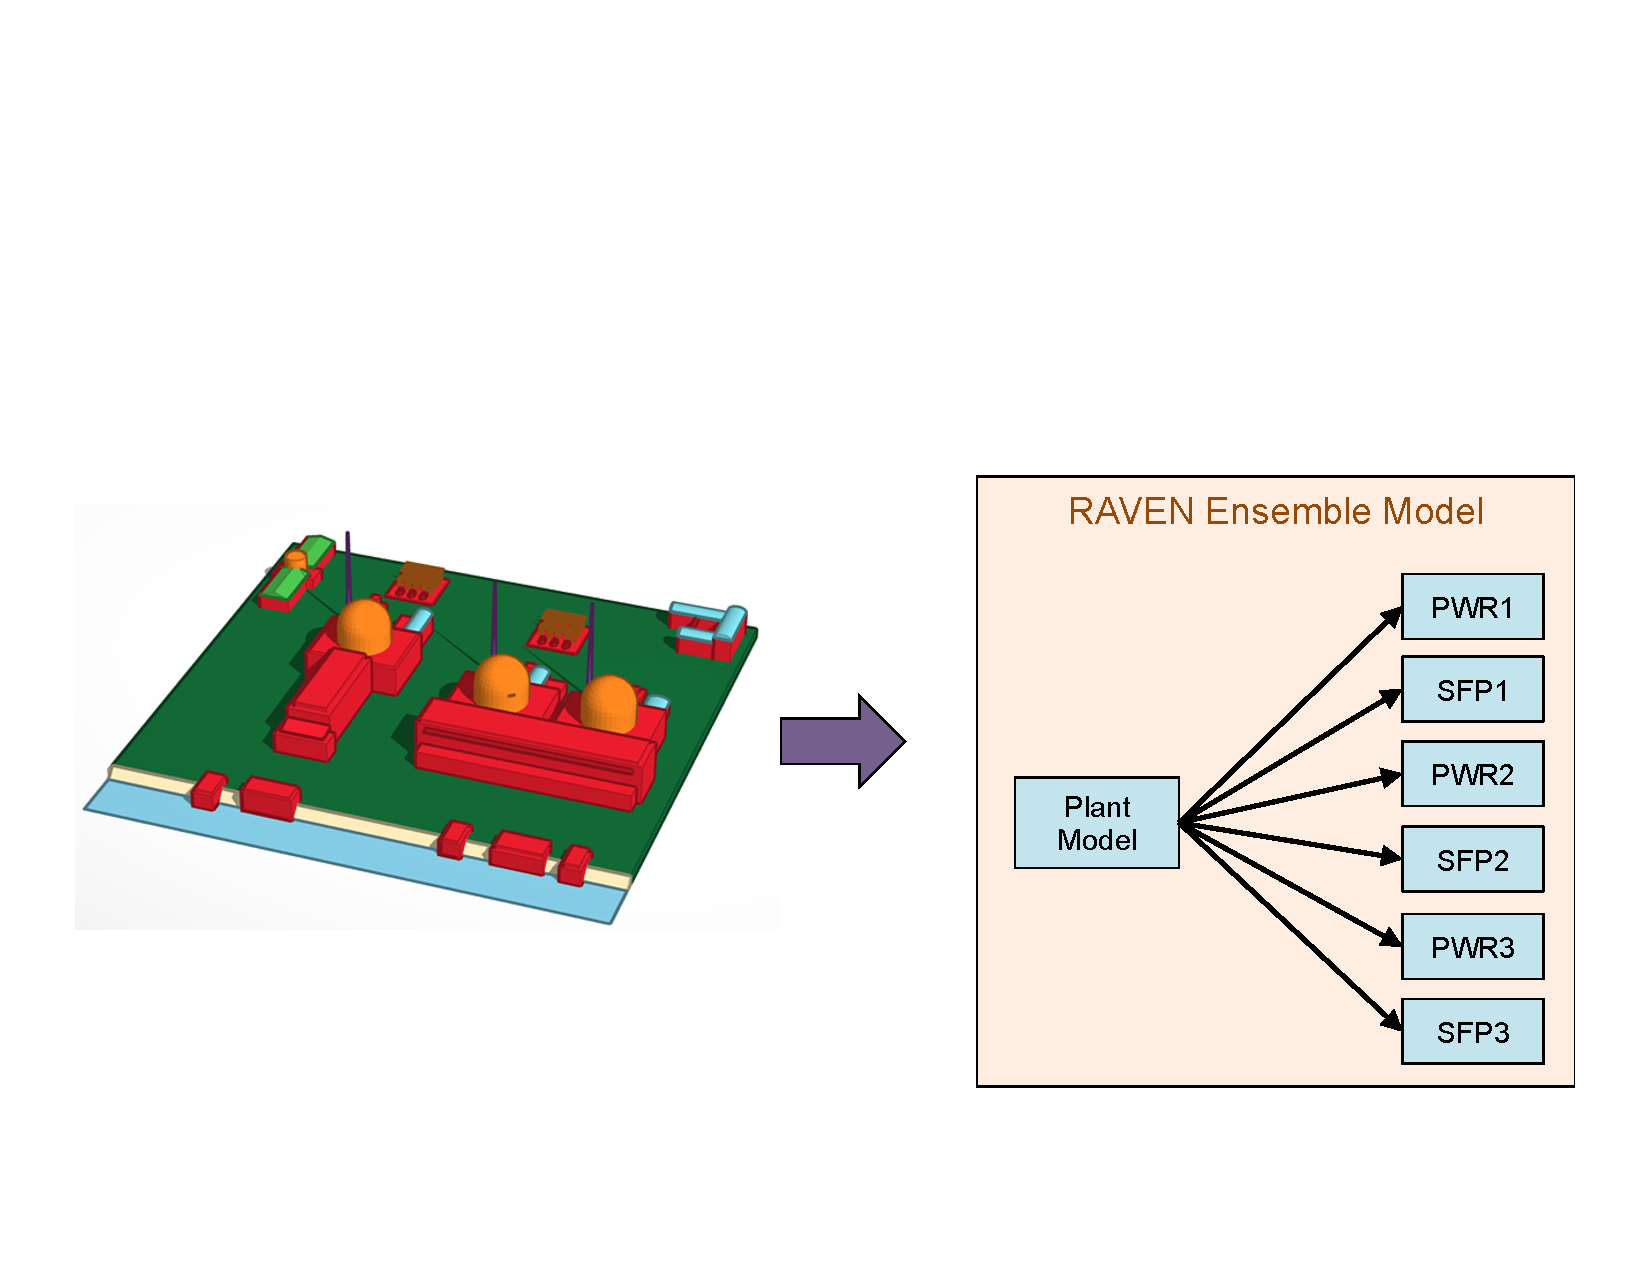
\includegraphics[scale=0.5]{ensembleModel.pdf}
    \caption{RAVEN ensemble model for the considered test case}
    \label{fig:ensembleModel}
\end{figure}

\subsection{System Models}
\label{sec:systemModels}
[CARLO]
\subsubsection{PWR1 and PWR3}

\subsubsection{PWR2}

\subsubsection{SFPs}

\subsection{Plant Model}
\label{sec:plantModel}
The plant model has been coded as a Python script and interfaced with RAVEN as an 
external model. Its main purpose is to determine timing and sequencing of events 
for all six system models (i.e., PWRs and SFPs) given the sampled values of the 
stochastic parameters.

\subsection{Human models}
[RON]

\subsection{Plant Stochastic Modeling}
For the scope of this analysis, we have identified 23 stochastic parameters. We have 
partition this list of parameters based on their area of interest.

Regarding the SFPs, we have have identified seismic induced rupture, i.e. a SFP LOCA, as 
element to include into the analysis. It has been modeled by choosing two stochastic 
parameters: time of  occurrence and size of the SFP LOCA. In this work we have identified 
with locaTimeSFP1, locaTimeSFP2 and locaTimeSFP3 as the time of occurrence of the SFP 
LOCAs while locaSizeSFP1, locaSizeSFP2 and locaSizeSFP3 represents the actual size of 
the SFP LOCAs.

Regarding the PWRs, we focused on two elements: lifetime of the batteries and the LOCA 
associated to the seal of the RCPs. Battery systems provides DC power to I\&C systems 
of the PWRs such as the control of the PORVs. DC systems are considered for only 
Unit 1 and Unit 3; since Unit 2 is in mid-loop operation mode, its DC systems are not 
considered.

For the EDGS, we have identified the following parameters: the probability to 
involuntary align the EDGS from Unit 2 to Unit 1, the time of occurrence of EDGS
involuntary alignment and time required to perform EDGS voluntary alignment.  

Each cross-tie, CST (between Unit 2 and Unit 3), AFW (between Unit 1 and Unit 3) 
and AC (between Unit 1 and Unit 1), has been considered in the analysis and, in 
particular, they have been modeled by assigning to each of them the time required 
to perform such cross-tie.

Regarding the recovery of each unit through the EPEs, we have modeled them by 
representing them with a single stochastic parameter which represents the
time to connect the EPE to its own unit.

Lastly, the recovery plan followed by the plant crew has been modeled using a single
parameter: recovery strategy (see Section~\cite{sec:accidentProgression}).

In addition to recovery strategy, we have given an additional degree of freedom on 
the actual procedure associated to the EPE for Unit 3. 
As indicated in Section~\ref{sec:EPEactions}, depending on the  recovery strategy, 
then the EPE connection on Unit 3 can be performed in different modes. 

A summary of the chosen stochastic parameters are listed in Table~\ref{tab:stochasticParameters} 
along a description and with their probabilistic distribution.

\begin{table}
  %\centering
  \begin{center}
      \begin{tabular}{ | l | p{5cm} | p{5cm} |}
        \hline
         Parameter          & Distribution & Description                      \\ \hline \hline
         AUXFWxtieTime      &              & Time to perform AFW cross-tie    \\ \hline
         CSTxtieTime        &              & Time to perform CST cross-tie    \\ \hline
         recoveryStrategy   &              & Recovery strategy to be followed \\ \hline
         EPETime1           &              & Time to connect EPE to Unit 1    \\ \hline
         EPETime2           &              & Time to connect EPE to Unit 2    \\ \hline
         EPETime3           &              & Time to connect EPE to Unit 3    \\ \hline
         EDGSinvolAlign     &              & Probability of occurrence for EDGS involuntary alignment   \\ \hline
         EDGSinvolAlignTime &              & Time of occurrence for EDGS involuntary alignment          \\ \hline
         EDGSswitchTime     &              & Time required to change EDGS alignment  \\ \hline
         ACxTieUnit12       &              & Time to perform AC cross-tie     \\ \hline
         batteryTime1       &              & Battery life for Unit 1          \\ \hline
         batteryTime3       &              & Battery life for Unit 3          \\ \hline
         locaTimePWR1       &              & Time of occurrence for PWR1 seal LOCA   \\ \hline
         locaTimePWR3       &              & Time of occurrence for PWR3 seal LOCA   \\ \hline
         locaSizeSFP1       &              & LOCA size for SFP1               \\ \hline
         locaSizeSFP2       &              & LOCA size for SFP1               \\ \hline
         locaSizeSFP3       &              & LOCA size for SFP1               \\ \hline    
         locaTimeSFP1       &              & Time of occurrence for SFP1 LOCA \\ \hline
         locaTimeSFP2       &              & Time of occurrence for SFP2 LOCA \\ \hline
         locaTimeSFP3       &              & Time of occurrence for SFP3 LOCA \\ \hline
         flex3Strategy13    &              & Type of EPE connection for Unit 3 during recovery strategy 1 and 3  \\ \hline
         flex3Strategy2     &              & Type of EPE connection for Unit 3 during recovery strategy 1 and 3  \\ 
        \hline
      \end{tabular}
  \end{center}
  \caption{Summary of the stochastic parameters chosen for the multi-unit analysis and their associated distribution}
  \label{tab:stochasticParameters}
\end{table}


